\chapter{Cloud Computing, Orchestration and Security}

\section{The Cloud Computing Model}
\begin{figure}[H]
    \centering
    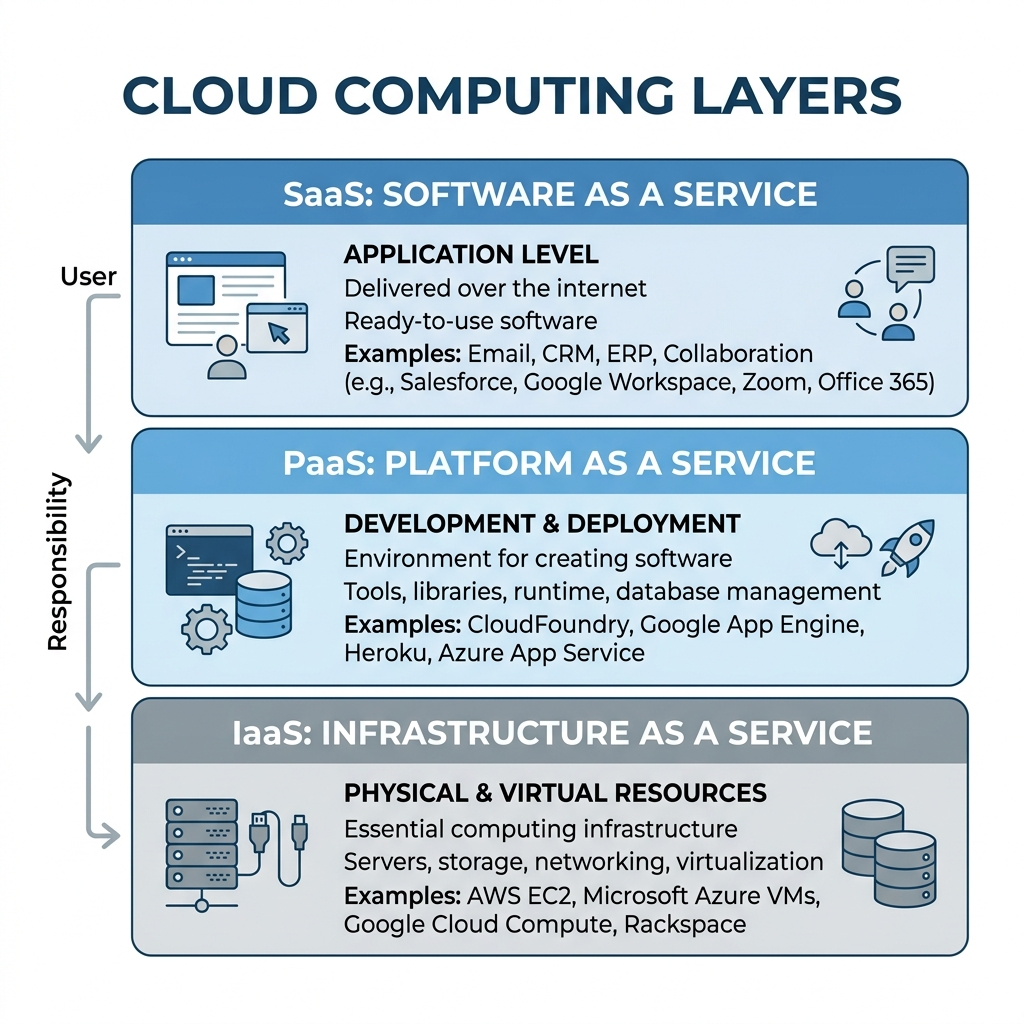
\includegraphics[width=0.8\textwidth]{images/cloud_computing.png}
    \caption{Abstract representation of Cloud Computing architecture layers.}
\end{figure}
Cloud computing represents not only a technological change, but a profound shift in the IT business model: moving from purchasing hardware (CapEx) to paying for the consumption of a service (OpEx).

\begin{tipbox}[The Challenges of Public Administration]
Building a cloud for a digital-native company or for the Public Administration (PA) are two opposing challenges. A startup operates in a \textbf{Greenfield} environment (starting from scratch with modern standards). The PA typically operates in a \textbf{Brownfield}: it must migrate decades-old applications and mainframes to the cloud without interrupting critical services to citizens. Furthermore, structural obstacles intervene:
\begin{itemize}
    \item \textbf{Governance:} Centralized model (more secure and economical on a national scale) vs Federated (politically preferred by local entities that do not want to cede control over their data).
    \item \textbf{Chargeback:} How to exactly allocate costs (internal billing) among different departments/ministries sharing the same hardware without generating disputes.
    \item \textbf{Procurement:} Purchasing physical hardware in PA on-premise clouds requires exhausting public tenders (with average delays of 1-2 years), making the purchased server already technologically obsolete by the time it is physically delivered to the datacenter.
\end{itemize}
\end{tipbox}

\subsection{Definition and Characteristics (NIST)}
According to NIST, the cloud is characterized by:
\begin{itemize}
    \item \textbf{On-demand self-service:} Autonomous provisioning by the customer without human intervention from the provider.
    \item \textbf{Broad network access:} Ubiquitous accessibility via standard network.
    \item \textbf{Resource pooling:} Shared resources in multi-tenant mode.
    \item \textbf{Rapid elasticity:} Ability to rapidly scale up and down (resources appear infinite to the consumer).
    \item \textbf{Measured service:} Pay-as-you-go model and continuous measurement of resources.
\end{itemize}

\subsection{Service Models}
\begin{itemize}
    \item \textbf{IaaS (Infrastructure as a Service):} The provider supplies "raw" or virtualized CPU, network, and storage. The consumer manages from the Operating System upwards.
    \item \textbf{PaaS (Platform as a Service):} The provider also manages the OS and runtime environment. The consumer only loads their application (e.g., managed databases, web apps).
    \item \textbf{SaaS (Software as a Service):} Everything is managed by the provider (e.g., Gmail, Microsoft 365). The user only uses the final software.
\end{itemize}

\section{Reference Architecture (Reference Model)}
The Reference Model is articulated in layers:
\begin{enumerate}
    \item \textbf{Physical Layer:} Physical hardware (Servers, Switches, Storage arrays). At this level operate the \textbf{Element Managers}, which are proprietary management interfaces provided by the manufacturer (e.g. the GUI of a single switch or an EMC array) that see \textit{only} their own physical device.
    \item \textbf{Virtual Layer:} Virtual machines, vSwitches, virtual LUNs. Abstracts the physical hardware providing flexible resource pools.
    \item \textbf{Control Layer:} Responsible for globally managing and grouping virtual resources. The \textbf{Unified Manager} operates here (e.g., VMware vCenter or Microsoft SCVMM), a super-manager that aggregates thousands of hosts ignoring hardware brand differences and allows the administrator to apply allocation \textit{policies} (absolute vs relative reservations) and over-allocation (Overbooking).
    \item \textbf{Orchestration Layer:} Automates complex workflows via scripts and asynchronous API calls. While the control layer executes a single primary task ("turn on VM"), the orchestrator coordinates an entire multi-step \textit{pipeline} ("create VM, configure vSwitch, allocate IP, install OS, install Database").
    \item \textbf{Service Layer:} Provides the \textit{Cloud Portal} and \textit{Service Catalog} in self-service mode, from which end users (tenants) order resources with a click, without having to open IT tickets.
\end{enumerate}

\subsection{Cloud Service Lifecycle}
Behind the scenes, the delivery of a cloud service passes through four mandatory macro-phases:
\begin{itemize}
    \item \textbf{Phase 1: Service Planning.} The IT architect defines the boundaries of the service, calculates the required resources and, above all, defines the \textbf{Billing Policy} (the exact billing metric, e.g., per allocated GB, per CPU-hour or per Giga of outgoing traffic).
    \item \textbf{Phase 2: Service Creation.} The orchestrator receives the order from the portal and converts it into dozens of concrete API calls to the infrastructure to build the service, allocating IP, disks and CPU.
    \item \textbf{Phase 3: Service Operation.} The service goes into production and is handed over to the tenant. It is constantly monitored by probes to verify compliance with SLAs (Quality of Service) and to quantify the consumed resources for billing purposes (Metering).
    \item \textbf{Phase 4: Service Termination.} At contract expiration or cancellation, the system must automatically deallocate all resources, irreversibly delete data (Secure Wipe) to protect the old tenant's privacy, and return IP addresses and storage to the available pool.
\end{itemize}

\begin{definitionbox}[SLA (Service Level Agreement) and Legal Clauses]
It is the binding contract between cloud provider and consumer that establishes the guaranteed service levels (uptime, performance, security). It includes measurement metrics and penalties (\textit{Service Credits}) in case of violation. Historically, SLAs hide complex clauses in favor of the provider: 
\begin{itemize}
    \item \textbf{Downtime vs User-minutes:} The calculation of downtime is not absolute. A failure of 10\% of the infrastructure might not violate the SLA if calculated on the total expected monthly "user-minutes".
    \item \textbf{Exclusions:} Scheduled maintenance (\textit{Scheduled Downtime}) or outages caused by customer misuse are excluded from penalties.
    \item \textbf{Lock-in:} Technical-legal difficulties in migrating one's data out without incurring enormous transfer costs (\textit{Egress}) or dependency on proprietary formats.
\end{itemize}
\end{definitionbox}

\section{Business Continuity and Data Protection}
The cloud assumes that hardware failures are physiological. The goal is to minimize the impact on the service (High Availability).
The main parameters are:
\begin{itemize}
    \item \textbf{RTO (Recovery Time Objective):} Time needed to restore the service in case of disaster.
    \item \textbf{RPO (Recovery Point Objective):} How far back in time data is lost in case of restoration. Determines backup frequency.
\end{itemize}

\subsection{Resilience Techniques and Geographical Limits}
To avoid \textbf{SPOFs (Single Points of Failure)}, multi-level redundancy techniques are used:
\begin{itemize}
    \item \textbf{Service Failover vs VM Replication:} Traditional \textit{Service Failover} (e.g. Windows Server Failover Cluster) relies on a passive secondary node; if the primary dies, the secondary mounts the shared storage and performs a slow cold reboot of the application (with an RTO of minutes). \textit{VM Replication} or \textbf{Continuous Data Protection (CDP)} operate instead at a lower level. A CDP injects a driver (\textit{Write Splitter}) into the hypervisor that bifurcates every I/O write: one copy goes to the local disk, the other via asynchronous network to the Disaster Recovery site. It uses a \textit{Journal Volume} to maintain a granular second-by-second timeline, allowing to "rewind" the entire VM in time to 5 seconds before a potential ransomware attack.
    \item \textbf{Active/Active vs Active/Passive:} The Active/Passive approach uses a standby secondary node. The Active/Active approach distributes the load simultaneously across multiple geographic datacenters, but encounters a severe physical limit dictated by the speed of light in optical fiber.
    \item \textbf{Synchronous vs Asynchronous Replication:} For two datacenters to operate in true Active/Active (without corrupting shared databases), storage replication must be \textbf{Synchronous} (the write is confirmed to the client only after both geographic sites have saved it). To do this without paralyzing applications, the latency time (\textit{Round-Trip Time}) between datacenters must not exceed \textbf{10-15 milliseconds}, which forces sites to be no more than $\sim$100-150 km apart from each other. For greater distances (e.g., between continents), it is mandatory to use \textbf{Asynchronous} replication (where there is a vulnerability window, RPO > 0), because waiting for the light signal would render the system unusable.
    \item \textbf{Availability Zones:} Division into distinct zones (often in different datacenters within the 15ms threshold) isolated from common failures (power, floods) but connected by dedicated optical fiber (Dark fiber) to appear as a single large logical infrastructure.
\end{itemize}

\subsection{Application Resiliency: Design for Failure}
Modern cloud architectures surrender to the statistical evidence that hardware will inevitably fail. Resilience is therefore abstracted and moved entirely to the software level (\textbf{Design for Failure}):
\begin{itemize}
    \item \textbf{Statelessness and Persistent State:} Containers and web servers must \textit{never} save local data. The persistent state is constantly offloaded to external databases or Object Storage (e.g., S3), allowing Kubernetes to "kill" and recreate an infected or failed application node in 1 second, without data loss and without causing interruptions to users.
    \item \textbf{Graceful Degradation:} If Netflix's sophisticated AI recommendation service fails in the cloud, the user interface should not generate a 500 error page. It must degrade the experience "gracefully", automatically serving a trivial generic pre-compiled static list of movies.
    \item \textbf{Retry Logic and Circuit Breaker:} Asynchronous API calls between cloud microservices will fail due to network timeouts or latency. Software patterns are implemented to retry (\textit{Exponential Backoff}) or "open the circuit" (\textit{Circuit Breaker}), completely disabling the problematic call to avoid bombarding and definitively bringing down an already congested microservice.
    \item \textbf{Event-Driven Architecture:} Decoupling via asynchronous queues (e.g. Kafka or RabbitMQ). If a database is temporarily overloaded by an unpredictable traffic spike, incoming writes accumulate patiently in the queue instead of failing, being processed as soon as the database recovers.
\end{itemize}

\section{Security}
Security in the cloud is based on the concept of \textbf{Trust} between customer and provider, built through visibility and control. The goal is to guarantee the \textbf{CIA} pillars (Confidentiality, Integrity, Availability).

\subsection{Classic Threats and Attacks}
Historically, datacenters had to defend against attacks aimed at the perimeter (Firewall). Classic threats include:
\begin{itemize}
    \item \textbf{Spoofing:} Forging identity (e.g., IP spoofing) to bypass ACLs.
    \item \textbf{Man-in-the-Middle (MitM) and Sniffing:} Unauthorized interception of traffic in transit.
    \item \textbf{Denial of Service (DDoS):} Saturation of resources (computational or bandwidth) to bring down service availability.
    \item \textbf{Phishing / Social Engineering:} Compromising the human factor to steal valid credentials.
\end{itemize}

\subsection{Identity and Policy Management (AAA and RBAC)}
Beyond perimeter defense, the vital foundation of cloud security in multi-tenant environments is the correct management of access and privileges:
\begin{itemize}
    \item \textbf{AAA Model:} Represents the fundamental security framework.
    \begin{itemize}
        \item \textit{Authentication (Who are you?):} Rigorous identity verification (e.g., via passwords, certificates or Multi-Factor Authentication).
        \item \textit{Authorization (What can you do?):} Evaluation and granting of the user's exact permissions on individual cloud resources.
        \item \textit{Accounting (What did you do?):} Tracking and immutable logging of every action (Audit Trail) for post-incident forensic analysis and billing purposes.
    \end{itemize}
    \item \textbf{RBAC (Role-Based Access Control):} In the cloud, permissions are almost never assigned to the individual user directly (it would be unmanageable). Logical \textbf{Roles} are created (e.g. "Storage Admin", "Auditor"). The user assumes the role or is associated with it. This system avoids the uncontrolled proliferation of privileges and ensures compliance with the \textit{Least Privilege} security principle (always and only provide the minimum privilege necessary to perform a task).
\end{itemize}

\subsection{Defense-in-Depth and Zero Trust Approach}
Since classic attacks have proven that a single secure perimeter does not exist and that threats also come from within (\textit{Insider Threat}), the classic model (based on a single external DMZ) is today replaced by \textbf{Zero Trust Architecture (ZTA)}. The principle is: "Never trust, always verify", relying on strong authentication and dynamic \textit{Micro-segmentation} before accessing every single workload.
The foundation of the security architecture is the \textbf{TCB (Trusted Computing Base)}, the set of critical components (e.g., hypervisor, BMC firmware), which if compromised inevitably bring down the entire chain of trust.

\subsection{Risk Management (GRC)}
Encompassed in the \textbf{GRC} (Governance, Risk management, Compliance) framework:
\begin{itemize}
    \item No system is 100\% inviolable. Risk Assessment evaluates the probability of an incident against the cost of the countermeasure.
    \item Compliance ensures adherence to regulations such as GDPR, NIS2, etc.
\end{itemize}
